% !TeX program = xelatex
\documentclass[a4paper,10pt]{article}

% ============================================================================
% ១. កញ្ចប់បណ្ណាល័យ និងការកំណត់ទំព័រ (Packages & Page Setup — តាមគំរូ ls_plan.tex)
% ============================================================================
\usepackage[a4paper, left=0.95cm, right=0.95cm, top=0.85cm, bottom=0.92cm, footskip=0.52cm]{geometry}
\usepackage{amsmath}
\usepackage{unicode-math}
\usepackage{fontspec}
\usepackage{longtable, array, multirow, colortbl}
\usepackage[table]{xcolor}
\usepackage{enumitem}
\usepackage{pifont}
\usepackage{fancyhdr}
\usepackage{tikz}
\usetikzlibrary{calc, arrows.meta, decorations.pathreplacing, patterns, positioning, babel}

\makeatletter
\let\@expl@@@mark@update@singlecol@structures@@\relax
\makeatother

% --- ប្រព័ន្ធស្វែងរកទីតាំងពុម្ពអក្សរស្វ័យប្រវត្តិ (Windows Local + Cloud Repo fonts/) ---
\providecommand{\NGSFindFonts}{%
  \IfFileExists{C:/Windows/Fonts/cambria.ttc}{%
    \def\NGSSysPath{C:/Windows/Fonts/}%
    \def\NGSUserPath{C:/Users/KIT/AppData/Local/Microsoft/Windows/Fonts/}%
  }{%
    \IfFileExists{./fonts/KhmerOSsiemreap.ttf}{\def\NGSSysPath{./fonts/}\def\NGSUserPath{./fonts/}}{%
    \IfFileExists{../fonts/KhmerOSsiemreap.ttf}{\def\NGSSysPath{../fonts/}\def\NGSUserPath{../fonts/}}{%
    \IfFileExists{../../fonts/KhmerOSsiemreap.ttf}{\def\NGSSysPath{../../fonts/}\def\NGSUserPath{../../fonts/}}{%
    \IfFileExists{../../../fonts/KhmerOSsiemreap.ttf}{\def\NGSSysPath{../../../fonts/}\def\NGSUserPath{../../../fonts/}}{%
    \IfFileExists{../../../../fonts/KhmerOSsiemreap.ttf}{\def\NGSSysPath{../../../../fonts/}\def\NGSUserPath{../../../../fonts/}}{%
    \IfFileExists{../../../../../fonts/KhmerOSsiemreap.ttf}{\def\NGSSysPath{../../../../../fonts/}\def\NGSUserPath{../../../../../fonts/}}{%
    \IfFileExists{../../../../../../fonts/KhmerOSsiemreap.ttf}{\def\NGSSysPath{../../../../../../fonts/}\def\NGSUserPath{../../../../../../fonts/}}{%
      \def\NGSSysPath{../../../../../../../fonts/}\def\NGSUserPath{../../../../../../../fonts/}%
    }}}}}}}%
  }%
}
\NGSFindFonts

% ============================================================================
% ២. កំណត់ពុម្ពអក្សរ (Fonts — តាមគំរូ ls_plan.tex)
% ============================================================================
\setmathfont[Path={\NGSSysPath}, FontIndex=1, Scale=1.02]{cambria.ttc}
\defaultfontfeatures{Ligatures=TeX}

\setmainfont[
  Path={\NGSUserPath},
  Extension=.ttf,
  Script=Khmer,
  BoldFont={KhmerOSsiemreap},
  BoldFeatures={FakeBold=1.8},
  ItalicFont={KhmerOSsiemreap},
  ItalicFeatures={FakeSlant=0.25},
  BoldItalicFont={KhmerOSsiemreap},
  BoldItalicFeatures={FakeBold=1.8, FakeSlant=0.25}
]{KhmerOSsiemreap}

\newfontfamily\muol[Path={\NGSUserPath}, Extension=.ttf, Script=Khmer]{KhmerOSmuollight}
\newfontfamily\Tacteing[Path={\NGSUserPath}, Extension=.TTF]{TACTENG}
\newfontfamily\TimesEn[Path={\NGSSysPath}, Extension=.ttf, BoldFont={timesbd}, ItalicFont={timesi}, BoldItalicFont={timesbi}]{times}
\newfontfamily\CalibriFont[Path={\NGSSysPath}, Extension=.ttf]{calibri}
\newfontfamily\CourierCirc[Path={\NGSSysPath}, Extension=.ttf]{cour}

\XeTeXlinebreaklocale "km"
\XeTeXlinebreakskip = 0pt plus 1pt minus 0.1pt

% ============================================================================
% ៣. ពណ៌ និងការតុបតែង (Colors & Styles)
% ============================================================================
\definecolor{stepbg}{HTML}{D9D9D9}
\definecolor{headgray}{HTML}{E6E6E6}
\definecolor{emphred}{HTML}{C00000}

\pagestyle{fancy}
\fancyhf{}
\renewcommand{\headrulewidth}{0pt}
\fancyfoot[R]{\CalibriFont\fontsize{9pt}{11pt}\selectfont\thepage}

\setlength{\parindent}{0pt}
\setlength{\parskip}{0pt}
\setlength{\tabcolsep}{4.5pt}
\setlength{\LTpre}{2pt}
\setlength{\LTpost}{2pt}

\newcolumntype{L}[1]{>{\raggedright\arraybackslash}p{#1}}
\newcolumntype{C}[1]{>{\centering\arraybackslash}p{#1}}

% ============================================================================
% ៤. ពាក្យបញ្ជាជំនួយ (Helper Macros)
% ============================================================================
\newcommand{\en}[1]{{\TimesEn #1}}
\newcommand{\enbf}[1]{{\TimesEn\bfseries #1}}
\newcommand{\khmflourish}{{\Tacteing\fontsize{15pt}{15pt}\selectfont 3}}
\newcommand{\wcirc}{{\CourierCirc\fontsize{9.5pt}{11pt}\selectfont o}}
\newcommand{\ditem}{{\fontsize{7.5pt}{10pt}\selectfont\ding{117}}\ }
\newcommand{\fiveE}[1]{\textcolor{emphred}{\CalibriFont\bfseries #1}}
\newcommand{\redsub}[1]{\textcolor{emphred}{#1}}
\newcommand{\timenote}[1]{\textcolor{emphred}{\textit{#1}}}
\newcommand{\stepheader}[1]{\multicolumn{3}{|c|}{\cellcolor{stepbg}\muol #1} \\ \hline}
\newcommand{\cfig}[1]{{\centering\vspace{3pt}#1\vspace{3pt}\par}}
\newcommand{\cnum}[1]{\mbox{\fontsize{10.5pt}{12pt}\selectfont\ding{\numexpr181+#1\relax}}}
\newcommand{\unit}[1]{\,\text{\en{#1}}}
\newcommand{\riel}{\,\text{៛}}
\newcommand{\usd}{\,\text{\en{\$}}}
\newcommand{\graybox}[1]{\colorbox{headgray}{\strut #1}}

% ============================================================================
% ៥. រូបភាព TikZ ស-ខ្មៅ សម្រាប់បង្រៀនលើក្ដារខៀន និងសន្លឹកកិច្ចការ (B&W Diagrams)
% ============================================================================

% ១. E1 Engage: គណនីសន្សំភ្លោះ A (សាមញ្ញ) ទល់នឹង B (សមាស) លើ 1 000 000៛ 2 ឆ្នាំ 10%
\newcommand{\figEngageINTThreeTwoSix}{%
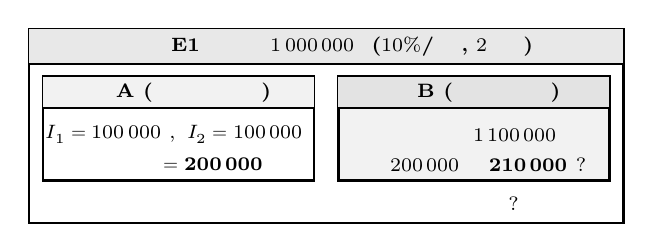
\begin{tikzpicture}[x=1cm, y=1cm, every node/.style={font=\scriptsize, text=black}]
  \draw[black, line width=0.9pt] (0,0) rectangle (7.55,2.46);
  \fill[gray!18] (0,2.02) rectangle (7.55,2.46);
  \draw[black, line width=0.6pt] (0,2.02) -- (7.55,2.02);
  \node at (3.775,2.24) {\textbf{បេសកកម្ម \en{E1}៖ គណនីភ្លោះ $1\,000\,000\riel$ ($10\%$/ឆ្នាំ, $2$ ឆ្នាំ)}};

  % Left: Account A
  \draw[black, line width=0.8pt] (0.18,0.54) rectangle (3.62,1.86);
  \fill[gray!10] (0.18,1.46) rectangle (3.62,1.86);
  \draw[black, line width=0.5pt] (0.18,1.46) -- (3.62,1.46);
  \node at (1.90,1.66) {\textbf{គណនី \en{A} (ដកការប្រាក់រាល់ឆ្នាំ)}};
  \node at (1.90,1.12) {$I_1 = 100\,000\riel, \ I_2 = 100\,000\riel$};
  \node at (1.90,0.74) {ការប្រាក់សរុប $= \mathbf{200\,000\riel}$};

  % Right: Account B
  \draw[black, line width=0.95pt, fill=gray!10] (3.93,0.54) rectangle (7.37,1.86);
  \fill[gray!22] (3.93,1.46) rectangle (7.37,1.86);
  \draw[black, line width=0.55pt] (3.93,1.46) -- (7.37,1.46);
  \node at (5.65,1.66) {\textbf{គណនី \en{B} (បូកការប្រាក់ចូលដើម)}};
  \node at (5.65,1.12) {ដើមឆ្នាំ២ ឡើងជា $1\,100\,000\riel$};
  \node at (5.65,0.74) {ស្មើ $200\,000\riel$ ឬ $\mathbf{210\,000\riel}$?};

  \node at (3.775,0.24) {\textbf{សំណួរគន្លឹះ៖} តើការប្រាក់ឆ្នាំទី១ អាចបង្កើតការប្រាក់នៅឆ្នាំទី២ ដែរឬទេ?};
\end{tikzpicture}}

% ២. E2 Explore: ដ្យាក្រាមព្រួញបន្តប្រាក់ដើមរបស់មីងសៅ (ទំ.៣៧ — 8 000 000៛, 15%, 2 ឆ្នាំ)
\newcommand{\figCarryLedgerINTThreeTwoSix}{%
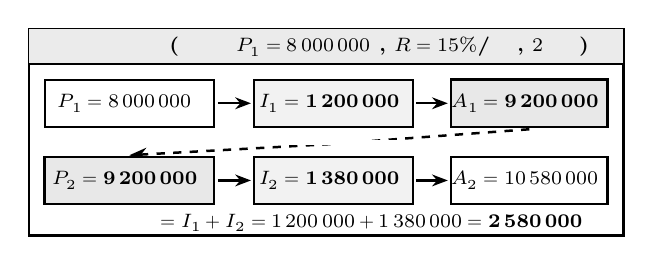
\begin{tikzpicture}[x=1cm, y=1cm, every node/.style={font=\scriptsize, text=black}]
  \draw[black, line width=0.9pt] (0,0) rectangle (7.55,2.62);
  \fill[gray!16] (0,2.18) rectangle (7.55,2.62);
  \draw[black, line width=0.6pt] (0,2.18) -- (7.55,2.18);
  \node at (3.775,2.40) {\textbf{ព្រួញបន្តប្រាក់ដើម (មីងសៅដាក់ $P_1 = 8\,000\,000\riel$, $R = 15\%$/ឆ្នាំ, $2$ ឆ្នាំ)}};

  % Year 1 row boxes
  \draw[black, line width=0.8pt] (0.20,1.38) rectangle (2.35,1.98);
  \node at (1.275,1.68) {$P_1 = 8\,000\,000\riel$};
  \draw[-{Stealth[length=2mm]}, black, line width=0.8pt] (2.40,1.68) -- (2.82,1.68);
  \draw[black, line width=0.8pt, fill=gray!10] (2.86,1.38) rectangle (4.88,1.98);
  \node at (3.87,1.68) {$I_1 = \mathbf{1\,200\,000\riel}$};
  \draw[-{Stealth[length=2mm]}, black, line width=0.8pt] (4.92,1.68) -- (5.32,1.68);
  \draw[black, line width=0.95pt, fill=gray!18] (5.36,1.38) rectangle (7.35,1.98);
  \node at (6.355,1.68) {$A_1 = \mathbf{9\,200\,000\riel}$};

  % Carry-forward diagonal arrow
  \draw[-{Stealth[length=2.2mm]}, black, dashed, line width=0.9pt] (6.355,1.35) -- (3.80,1.16) -- (1.275,1.02);
  \node[fill=white, inner sep=1pt] at (3.95,1.18) {\textbf{ក្លាយជាប្រាក់ដើមថ្មីឆ្នាំទី២}};

  % Year 2 row boxes
  \draw[black, line width=0.95pt, fill=gray!18] (0.20,0.40) rectangle (2.35,1.00);
  \node at (1.275,0.70) {$P_2 = \mathbf{9\,200\,000\riel}$};
  \draw[-{Stealth[length=2mm]}, black, line width=0.8pt] (2.40,0.70) -- (2.82,0.70);
  \draw[black, line width=0.8pt, fill=gray!10] (2.86,0.40) rectangle (4.88,1.00);
  \node at (3.87,0.70) {$I_2 = \mathbf{1\,380\,000\riel}$};
  \draw[-{Stealth[length=2mm]}, black, line width=0.8pt] (4.92,0.70) -- (5.32,0.70);
  \draw[black, line width=0.95pt] (5.36,0.40) rectangle (7.35,1.00);
  \node at (6.355,0.70) {$A_2 = 10\,580\,000\riel$};

  \node at (3.775,0.16) {ការប្រាក់សមាសសរុប $= I_1 + I_2 = 1\,200\,000 + 1\,380\,000 = \mathbf{2\,580\,000\riel}$};
\end{tikzpicture}}

% ៣. E3 Explain: ប្រៀបធៀបការប្រាក់សាមញ្ញ ទល់នឹង ការប្រាក់សមាស
\newcommand{\figCompareSimpleCompoundINTThreeTwoSix}{%
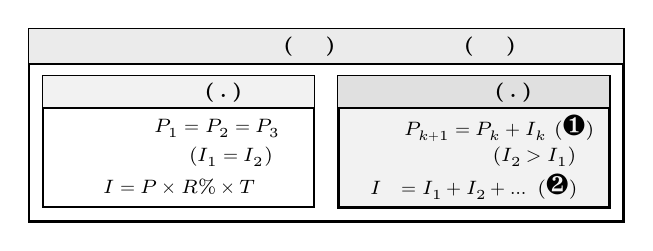
\begin{tikzpicture}[x=1cm, y=1cm, every node/.style={font=\scriptsize, text=black}]
  \draw[black, line width=0.9pt] (0,0) rectangle (7.55,2.44);
  \fill[gray!16] (0,2.00) rectangle (7.55,2.44);
  \draw[black, line width=0.6pt] (0,2.00) -- (7.55,2.00);
  \node at (3.775,2.22) {\textbf{ប្រៀបធៀប៖ ការប្រាក់សាមញ្ញ (ដើមថេរ) ទល់នឹង ការប្រាក់សមាស (ដើមកើន)}};

  % Left: Simple
  \draw[black, line width=0.8pt] (0.18,0.18) rectangle (3.62,1.84);
  \fill[gray!10] (0.18,1.44) rectangle (3.62,1.84);
  \draw[black, line width=0.5pt] (0.18,1.44) -- (3.62,1.44);
  \node at (1.90,1.64) {\textbf{ការប្រាក់សាមញ្ញ (២.៥)}};
  \node at (1.90,1.18) {ប្រាក់ដើមថេរ៖ $P_1 = P_2 = P_3$};
  \node at (1.90,0.82) {ការប្រាក់ស្មើៗគ្នា ($I_1 = I_2$)};
  \node at (1.90,0.44) {$I = P\times R\%\times T$};

  % Right: Compound
  \draw[black, line width=0.95pt, fill=gray!10] (3.93,0.18) rectangle (7.37,1.84);
  \fill[gray!24] (3.93,1.44) rectangle (7.37,1.84);
  \draw[black, line width=0.55pt] (3.93,1.44) -- (7.37,1.44);
  \node at (5.65,1.64) {\textbf{ការប្រាក់សមាស (២.៦)}};
  \node at (5.65,1.18) {ដើមថ្មី៖ $P_{k+1} = P_k + I_k$ (\cnum{1})};
  \node at (5.65,0.82) {ការប្រាក់កើនរាល់ឆ្នាំ ($I_2 > I_1$)};
  \node at (5.65,0.44) {$I_{\text{សមាស}} = I_1 + I_2 + \dots$ (\cnum{2})};
\end{tikzpicture}}

% ៤. E4 Elaborate: លំហាត់គំរូទី២ (ទំ.៣៨ — បន្តដើមប្រចាំឆមាស T = 1/2 ឆ្នាំ)
\newcommand{\figSemiannualINTThreeTwoSix}{%
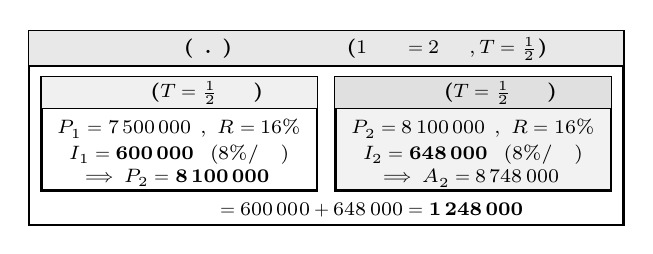
\begin{tikzpicture}[x=1cm, y=1cm, every node/.style={font=\scriptsize, text=black}]
  \draw[black, line width=0.9pt] (0,0) rectangle (7.55,2.46);
  \fill[gray!18] (0,2.02) rectangle (7.55,2.46);
  \draw[black, line width=0.6pt] (0,2.02) -- (7.55,2.02);
  \node at (3.775,2.24) {\textbf{លំហាត់គំរូទី២ (ទំ.៣៨)៖ បន្តដើមប្រចាំឆមាស ($1\text{ ឆ្នាំ} = 2\text{ ឆមាស}, T=\tfrac{1}{2}$)}};

  % Sem 1
  \draw[black, line width=0.8pt] (0.16,0.44) rectangle (3.66,1.88);
  \fill[gray!12] (0.16,1.48) rectangle (3.66,1.88);
  \draw[black, line width=0.55pt] (0.16,1.48) -- (3.66,1.48);
  \node at (1.91,1.68) {\textbf{ឆមាសទី ១ ($T = \tfrac{1}{2}\text{ ឆ្នាំ}$)}};
  \node at (1.91,1.22) {$P_1 = 7\,500\,000\riel, \ R = 16\%$};
  \node at (1.91,0.90) {$I_1 = \mathbf{600\,000\riel}$ ($8\%$/ឆមាស)};
  \node at (1.91,0.60) {$\implies P_2 = \mathbf{8\,100\,000\riel}$};

  % Sem 2
  \draw[black, line width=0.95pt, fill=gray!10] (3.89,0.44) rectangle (7.39,1.88);
  \fill[gray!24] (3.89,1.48) rectangle (7.39,1.88);
  \draw[black, line width=0.6pt] (3.89,1.48) -- (7.39,1.48);
  \node at (5.64,1.68) {\textbf{ឆមាសទី ២ ($T = \tfrac{1}{2}\text{ ឆ្នាំ}$)}};
  \node at (5.64,1.22) {$P_2 = 8\,100\,000\riel, \ R = 16\%$};
  \node at (5.64,0.90) {$I_2 = \mathbf{648\,000\riel}$ ($8\%$/ឆមាស)};
  \node at (5.64,0.60) {$\implies A_2 = 8\,748\,000\riel$};

  \node at (3.775,0.20) {ការប្រាក់សមាសសរុប $= 600\,000 + 648\,000 = \mathbf{1\,248\,000\riel}$};
\end{tikzpicture}}

% ៥. E5 Evaluate: ជម្រើសវិនិច្ឆ័យ A-D (ដាក់ប្រាក់ 2 000 000៛ អត្រា 10%/ឆ្នាំ រយៈពេល 2 ឆ្នាំ ការប្រាក់សមាស)
\newcommand{\figExitINTThreeTwoSix}{%
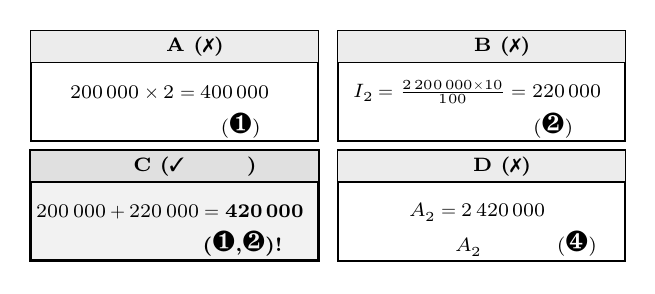
\begin{tikzpicture}[x=1cm, y=1cm, every node/.style={font=\scriptsize, text=black}]
  % A
  \draw[black, line width=0.8pt] (0,1.52) rectangle (3.65,2.92);
  \fill[gray!15] (0,2.52) rectangle (3.65,2.92);
  \draw[black, line width=0.55pt] (0,2.52) -- (3.65,2.52);
  \node at (1.825,2.72) {\textbf{ជម្រើស \en{A} (\ding{55})}};
  \node at (1.825,2.14) {$200\,000\times 2 = 400\,000\riel$};
  \node at (1.825,1.72) {ច្រឡំគិតការប្រាក់សាមញ្ញ (\cnum{1})};

  % B
  \draw[black, line width=0.8pt] (3.90,1.52) rectangle (7.55,2.92);
  \fill[gray!15] (3.90,2.52) rectangle (7.55,2.92);
  \draw[black, line width=0.55pt] (3.90,2.52) -- (7.55,2.52);
  \node at (5.725,2.72) {\textbf{ជម្រើស \en{B} (\ding{55})}};
  \node at (5.725,2.14) {$I_2 = \tfrac{2\,200\,000\times 10}{100} = 220\,000\riel$};
  \node at (5.725,1.72) {ភ្លេចបូកការប្រាក់ឆ្នាំទី១ (\cnum{2})};

  % C (Correct)
  \draw[black, line width=1.1pt, fill=gray!10] (0,0) rectangle (3.65,1.40);
  \fill[gray!24] (0,1.00) rectangle (3.65,1.40);
  \draw[black, line width=0.6pt] (0,1.00) -- (3.65,1.00);
  \node at (1.825,1.20) {\textbf{ជម្រើស \en{C} (\ding{51} ត្រឹមត្រូវ)}};
  \node at (1.825,0.62) {$200\,000 + 220\,000 = \mathbf{420\,000\riel}$};
  \node at (1.825,0.22) {\textbf{បន្តដើម និងបូកសរុបត្រូវ (\cnum{1},\cnum{2})!}};

  % D
  \draw[black, line width=0.8pt] (3.90,0) rectangle (7.55,1.40);
  \fill[gray!15] (3.90,1.00) rectangle (7.55,1.40);
  \draw[black, line width=0.55pt] (3.90,1.00) -- (7.55,1.00);
  \node at (5.725,1.20) {\textbf{ជម្រើស \en{D} (\ding{55})}};
  \node at (5.725,0.62) {$A_2 = 2\,420\,000\riel$};
  \node at (5.725,0.22) {ច្រឡំប្រាក់សរុប $A_2$ ជាការប្រាក់ (\cnum{4})};
\end{tikzpicture}}

% ============================================================================
% ចាប់ផ្ដើមឯកសារ (Document Body)
% ============================================================================
\begin{document}
\fontsize{10pt}{15.2pt}\selectfont

% -------------------- ក្បាលកិច្ចតែងការ (Header) --------------------
\begin{center}
  {\muol\fontsize{11pt}{16pt}\selectfont ព្រះរាជាណាចក្រកម្ពុជា}\\[2pt]
  {\muol\fontsize{10pt}{15pt}\selectfont ជាតិ សាសនា ព្រះមហាក្សត្រ}\\[1pt]
  \khmflourish
\end{center}

\vspace{-24pt}
{\muol\fontsize{9.5pt}{12.5pt}\selectfont
មន្ទីរអប់រំ យុវជន និងកីឡា ខេត្តកំពង់ធំ\\
ការិយាល័យអប់រំ យុវជន និងកីឡា ស្រុកកំពង់ស្វាយ\\
អនុវិទ្យាល័យព្រះក្រសាំង}

\vspace{1pt}
\begin{center}
  {\muol\fontsize{10pt}{14pt}\selectfont កិច្ចតែងការបង្រៀន}
\end{center}
\vspace{0pt}

% -------------------- ព័ត៌មានទូទៅ (Metadata) --------------------
{\renewcommand{\arraystretch}{0.98}
\hspace*{3.1cm}%
\begin{tabular}{@{}l l L{11.0cm}@{}}
  - \hspace{0.35cm} មុខវិជ្ជា & : & គណិតវិទ្យា ថ្នាក់ទី៨ (ពីជគណិត) \\
  - \hspace{0.35cm} ចំណងជើងមេរៀន & : & មេរៀនទី៣៖ ទំហំសមាមាត្រនិងភាគរយ \\
  - \hspace{0.35cm} ចំណងជើងរង & : & ២.៦. ការប្រាក់សមាស (ទំ.៣៧–៣៨, ៤២) \\
  - \hspace{0.35cm} រយៈពេល & : & ១ ម៉ោងសិក្សា (៥០ នាទី) \\
  - \hspace{0.35cm} បង្រៀនដោយ & : & ហុក ប៊ុនថែន \\
  - \hspace{0.35cm} កាលបរិច្ឆេទ & : & ថ្ងៃពុធ ទី២៥ ខែវិច្ឆិកា ឆ្នាំ២០២៦ \\
\end{tabular}

\vspace{2pt}

% -------------------- I. វត្ថុបំណង --------------------
\textbf{I.} {\muol វត្ថុបំណង}\\[1pt]
\hspace*{0.45cm}%
\begin{tabular}{@{}l l L{14.85cm}@{}}
  \wcirc \hspace{0.25cm} វិជ្ជាសម្បទា & : & សិស្សប្រាប់និយមន័យនៃការប្រាក់សមាស (ការបន្ថែមការប្រាក់កន្លងទៅលើប្រាក់ដើមដើម្បីបង្កើតប្រាក់ដើមថ្មីសម្រាប់គិតការប្រាក់ដំណាក់បន្ទាប់) និងប្រាប់ភាពខុសគ្នារវាងការប្រាក់សាមញ្ញនិងការប្រាក់សមាសបានត្រឹមត្រូវ ។ \\
  \wcirc \hspace{0.25cm} បំណិនសម្បទា & : & សិស្សគណនាការប្រាក់សមាស និងប្រាក់សរុបតាមតារាងបន្តប្រាក់ដើមប្រចាំឆ្នាំ និងប្រចាំឆមាស ($T = \frac{1}{2}$ ឆ្នាំ) លើសន្លឹកកិច្ចការ (ទំ.៣៧–៣៨) បានត្រឹមត្រូវ ។ \\
  \wcirc \hspace{0.25cm} ចរិយាសម្បទា & : & សិស្សយល់តម្លៃនៃការសន្សំប្រាក់រយៈពេលវែងតាមប្រព័ន្ធធនាគារ និងមានការប្រុងប្រយ័ត្នខ្ពស់ចំពោះបំណុលការប្រាក់បន្តដើមក្នុងជីវភាពរស់នៅ ។ \\
\end{tabular}

\vspace{2pt}

% -------------------- II. សម្ភារៈឧបទេស --------------------
\textbf{II.} {\muol សម្ភារៈឧបទេស}\\[1pt]
\hspace*{0.55cm}$\bullet$ \hspace{0.35cm} សៀវភៅសិក្សាគោលថ្នាក់ទី៨ (ទំ.៣៧–៣៨, ៤២) ក្ដារខៀន ដីស/ហ្វឺត បន្ទាត់ត្រង់ និង\textbf{សន្លឹកកិច្ចការសិស្សបំពេញចន្លោះ ស-ខ្មៅ} (\en{Printable\_Materials\_INT326} ទំព័រ ១–២ សម្រាប់សិស្ស និងទំព័រ ៣ ប្លង់ក្ដារខៀន/ចម្លើយគ្រូ — គ្មានប្រើ \en{LCD})

\vspace{2pt}

% -------------------- III. វិធីសាស្រ្តបង្រៀន --------------------
\textbf{III.} {\muol វិធីសាស្រ្តបង្រៀន}\\[1pt]
\hspace*{0.45cm}%
\begin{tabular}{@{}l l L{14.85cm}@{}}
  $\bullet$ \hspace{0.25cm} គោលវិធី & : & សិស្សមជ្ឈមណ្ឌល (សន្លឹកកិច្ចការបំពេញចន្លោះជាគោល + ការពិភាក្សាជាក្រុមតូច ៣ នាក់) \\
  $\bullet$ \hspace{0.25cm} យុទ្ធវិធីបង្រៀន & : & គំរូស្ថាបនានិយម \en{5Es} រួមបញ្ចូល \textbf{តារាងព្រួញបន្តប្រាក់ដើម (\en{Carry-Forward Ledger})} និង \textbf{ការប្រៀបធៀបសាមញ្ញ ទល់នឹង សមាស} \\
\end{tabular}
}

\vspace{2pt}

% -------------------- IV. ដំណើរការបង្រៀន --------------------
\textbf{IV.} {\muol ដំណើរការបង្រៀន}

\vspace{1pt}
{\renewcommand{\arraystretch}{1.12}
\begin{longtable}{|L{5.50cm}|L{7.90cm}|L{4.80cm}|}
\hline
\multicolumn{1}{|c|}{\cellcolor{headgray}\muol សកម្មភាពគ្រូ} &
\multicolumn{1}{c|}{\cellcolor{headgray}\muol ខ្លឹមសារមេរៀន} &
\multicolumn{1}{c|}{\cellcolor{headgray}\muol សកម្មភាពសិស្ស} \\
\endhead
\hline
\endfoot

% ==================== ជំហានទី១ (2min) ====================
\stepheader{ជំហានទី១ \enbf{(}រដ្ឋបាលថ្នាក់\enbf{)}}
$\bullet$ ពិនិត្យវត្តមាន អនាម័យ និងសណ្ដាប់ធ្នាប់ថ្នាក់រៀន \par
$\bullet$ រៀបចំក្រុមតូច ៣ នាក់តាមតុ និងចែក\textbf{សន្លឹកកិច្ចការសិស្ស (\en{INT326} ទំព័រ ១–២)}
&
$\bullet$ រដ្ឋបាលថ្នាក់ អនាម័យ និងវិន័យសិក្សា \par
$\bullet$ ចែកសន្លឹកកិច្ចការម្នាក់ ១ សន្លឹក សម្រាប់បំពេញតាមដំណាក់កាល \en{E1--E5}
&
$\circ$ ប្រធានថ្នាក់រាយការណ៍វត្តមានសិស្ស \par
$\circ$ ទទួលសន្លឹកកិច្ចការ សរសេរឈ្មោះ និងអង្គុយតាមក្រុម ៣ នាក់ \\
\hline

% ==================== ជំហានទី២ (9min: កំណែ <=3m + រំលឹក 3m + E1 3m) ====================
\stepheader{ជំហានទី២ \enbf{(}កិច្ចការផ្ទះ \enbf{+} ទំនាក់ទំនងមេរៀនថ្មី\enbf{)}}
\ditem \textbf{កំណែកិច្ចការផ្ទះ ($\le\text{\enbf{3\,min}}$)} \par
$\bullet$ ហៅសិស្ស ២ នាក់ឡើងកែលំហាត់ទំ.៤២ លេខ ១៦ និងលំហាត់ ៩ ខែ លើក្ដារខៀន
&
{\centering\redsub{កំណែកិច្ចការផ្ទះមេរៀនមុន (ទំ.៤២ \#16 និងលំហាត់ ៩ ខែ)}\par}
$\bullet$ \textbf{\#16 (ទំ.៤២)៖} អត្រាថយ $15\% - 13\% = 2\%$ ត្រូវនឹង $200\,000\riel \implies$ ប្រាក់ដើម $P = \frac{200\,000\times 100}{2} = \mathbf{10\,000\,000\riel}$ \par
$\bullet$ \textbf{លំហាត់ ៩ ខែ៖} $T = \frac{9}{12} = \frac{3}{4}$ ឆ្នាំ $\implies I = \mathbf{360\,000\riel}$, $A = \mathbf{6\,360\,000\riel}$
&
$\circ$ ផ្ទៀងចម្លើយ និងកែតម្រូវចូលសៀវភៅកិច្ចការផ្ទះ \\[3pt]

\ditem \textbf{រំលឹកមេរៀនទាក់ទង (\enbf{3min})} \par
$\bullet$ សួរ៖ «បើដាក់ប្រាក់ $P$ រយៈពេល $1$ ឆ្នាំ តើ $T$ និង $I$ ស្មើប៉ុន្មាន?»
&
{\centering\redsub{រំលឹកការប្រាក់ក្នុង ១ ឆ្នាំ និង ១ ឆមាស (២.៥)}\par}
$\bullet$ រយៈពេល $1\text{ ឆ្នាំ} \implies T = 1 \implies I = \tfrac{P\times R}{100}$
&
$\circ$ ឆ្លើយ៖ «$T=1 \implies I = \frac{P\times R}{100}$!» \\[3pt]

$\bullet$ សួរបន្ត៖ «ចុះបើដាក់ $1$ ឆមាស ($6$ ខែ) តើ $T$ ស្មើប៉ុន្មានឆ្នាំ?»
&
$\bullet$ រយៈពេល $1\text{ ឆមាស} = 6\text{ ខែ} \implies T = \tfrac{1}{2}\text{ ឆ្នាំ} \implies I = \tfrac{P\times R}{100}\times \tfrac{1}{2}$
&
$\circ$ ឆ្លើយ៖ «$1$ ឆមាស $T=\frac{1}{2}$ ឆ្នាំ!» \\[3pt]

\fiveE{E1 - Engage (3min)} \timenote{(កុំទាន់ផ្ដល់ចម្លើយ)} \par
\ditem \textbf{បេសកកម្មគណនីសន្សំភ្លោះ \en{A} និង \en{B} (សន្លឹកកិច្ចការ \en{E1})} \par
$\bullet$ ឱ្យសិស្សអានប្រអប់ \en{E1} ហើយគូសជ្រើសរើសរវាង \textbf{$200\,000\riel$} និង \textbf{$210\,000\riel$}
&
\redsub{បេសកកម្ម \en{E1}៖ គណនីសន្សំភ្លោះ $1\,000\,000\riel$ រយៈពេល $2$ ឆ្នាំ ($10\%$/ឆ្នាំ)} \par
បងប្អូនភ្លោះពីរនាក់ដាក់ប្រាក់ $1\,000\,000\riel$ ម្នាក់ ៖ គណនី \en{A} ដកការប្រាក់រាល់ឆ្នាំបាន $200\,000\riel$ ឯគណនី \en{B} ទុកការប្រាក់ឆ្នាំទី១ បូកចូលប្រាក់ដើម! \par
$\bullet$ នៅចុងឆ្នាំទី២ តើគណនី \en{B} បានការប្រាក់ $200\,000\riel$ ដូចគ្នា ឬបាន $210\,000\riel$?
&
$\circ$ ពិភាក្សាជាគូ និងគូស \ding{51} ក្នុងប្រអប់ \en{E1} លើសន្លឹកកិច្ចការ \\[3pt]

&
\cfig{\figEngageINTThreeTwoSix}
& \\
\hline

% ==================== ជំហានទី៣ (17min: E2 11m + E3 6m) ====================
\stepheader{ជំហានទី៣ \enbf{(}ខ្លឹមសារមេរៀនថ្មី\enbf{)}}
\fiveE{E2 - Explore (11min)} \par
$\bullet$ សរសេរចំណងជើងរង \textbf{២.៦. ការប្រាក់សមាស} លើក្ដារខៀន \par
\ditem \textbf{សកម្មភាព ១៖ តារាងព្រួញបន្តដើមរបស់មីងសៅ (\enbf{5min}, សន្លឹកកិច្ចការ \en{E2-A})} \par
$\bullet$ ឱ្យសិស្សបំពេញតារាងឆ្នាំទី១ និងទី២ នៃឧទាហរណ៍មីងសៅ (សៀវភៅទំ.៣៧)
&
មេរៀនទី៣ \quad {\muol ទំហំសមាមាត្រនិងភាគរយ \enbf{(}ត\enbf{)}} \par
២.៦. ការប្រាក់សមាស \par
$\bullet$ \textbf{ឧទាហរណ៍ (ទំ.៣៧ — មីងសៅដាក់ប្រាក់ $8\,000\,000\riel, R=15\%, 2$ ឆ្នាំ)៖} \par
\hspace*{0.2cm}-- \textbf{ឆ្នាំទី១៖} $P_1 = 8\,000\,000\riel \implies I_1 = \dfrac{8\,000\,000\times 15}{100} = 1\,200\,000\riel$ \par
\hspace*{0.2cm}-- \textbf{ដើមឆ្នាំទី២៖} $P_2 = 8\,000\,000 + 1\,200\,000 = 9\,200\,000\riel$ \par
\hspace*{0.2cm}-- \textbf{ឆ្នាំទី២៖} $I_2 = \dfrac{9\,200\,000\times 15}{100} = 1\,380\,000\riel$ \par
\hspace*{0.2cm}-- \textbf{ការប្រាក់សមាសសរុប៖} $1\,200\,000 + 1\,380\,000 = \mathbf{2\,580\,000\riel}$
&
$\circ$ បំពេញតារាងបន្តដើមលើសន្លឹកកិច្ចការ \en{E2-A} ឃើញការប្រាក់សមាស $2\,580\,000\riel$ (លើសសាមញ្ញ $180\,000\riel$) \\[3pt]

&
\cfig{\figCarryLedgerINTThreeTwoSix}
& \\[3pt]

\ditem \textbf{សកម្មភាព ២៖ លំហាត់គំរូទី ១ រយៈពេល ៣ ឆ្នាំ (\enbf{6min}, សន្លឹកកិច្ចការ \en{E2-B})} \par
$\bullet$ ឱ្យសិស្សបន្តបំពេញតារាង ៣ ឆ្នាំ របស់ទ្រាចាន់ និងមីងស្រី (សៀវភៅទំ.៣៧–៣៨)
&
$\bullet$ \textbf{លំហាត់គំរូទី ១ (ទំ.៣៧–៣៨ — ទ្រាចាន់ឱ្យខ្ចី $3\,000\,000\riel, R=20\%, 3$ ឆ្នាំ)៖} \par
\hspace*{0.2cm}-- ឆ្នាំទី១៖ $P_1 = 3\,000\,000\riel \implies I_1 = 600\,000\riel \implies P_2 = 3\,600\,000\riel$ \par
\hspace*{0.2cm}-- ឆ្នាំទី២៖ $P_2 = 3\,600\,000\riel \implies I_2 = 720\,000\riel \implies P_3 = 4\,320\,000\riel$ \par
\hspace*{0.2cm}-- ឆ្នាំទី៣៖ $P_3 = 4\,320\,000\riel \implies I_3 = 864\,000\riel$ \par
\hspace*{0.2cm}$\implies$ ការប្រាក់សមាសសរុប $= 600\,000 + 720\,000 + 864\,000 = \mathbf{2\,184\,000\riel}$
&
$\circ$ គណនាតាមតារាង ៣ ដំណាក់លើសន្លឹកកិច្ចការ \en{E2-B} ឃើញ $2\,184\,000\riel$ \\[3pt]

% --- E3 Explain (6min) ---
\fiveE{E3 - Explain (6min)} \par
$\bullet$ ដឹកនាំសិស្សសង្ខេបនិយមន័យ\textbf{ការប្រាក់សមាស} (ទំ.៣៧)
&
$\bullet$ \textbf{និយមន័យការប្រាក់សមាស (ទំ.៣៧)៖} រាល់ដំណាច់ឆ្នាំ (ឬឆមាស) គេបូកការប្រាក់កន្លងទៅចូលនឹងប្រាក់ដើម ដើម្បីបាន\textbf{ប្រាក់ដើមថ្មី} សម្រាប់គិតការប្រាក់ដំណាក់បន្ទាប់តាមអត្រាដដែល ។
&
$\circ$ បំពេញប្រអប់និយមន័យលើសន្លឹកកិច្ចការ \en{E3} \\[3pt]

$\bullet$ កត់ត្រារូបមន្តបន្តប្រាក់ដើម និងការប្រាក់សមាសសរុប
&
$\bullet$ \textbf{រូបមន្តបន្តប្រាក់ដើម និងការប្រាក់សរុប៖} \par
\hspace*{0.15cm}\graybox{$P_{k+1} = P_k + I_k$} \quad និង \quad \graybox{$I_{\text{សមាស}} = I_1 + I_2 + \dots + I_n = A_n - P_1$}
&
$\circ$ បំពេញរូបមន្តលើសន្លឹកកិច្ចការ \en{E3} \\[3pt]

&
\cfig{\figCompareSimpleCompoundINTThreeTwoSix}
& \\[3pt]

$\bullet$ ភ្ជាប់\textbf{ធនាគារហេតុផល \cnum{1}--\cnum{4}} លើក្ដារខៀន និងសន្លឹកកិច្ចការ
&
\textbf{ធនាគារហេតុផល (\en{Warrant Bank})៖} \par
\cnum{1} \textbf{បន្តប្រាក់ដើមថ្មី៖} រាល់ដំណាក់ $P_{\text{ថ្មី}} = P_{\text{ចាស់}} + I_{\text{មុន}}$ (កុំប្រើ $P_1$ ដដែល!) \par
\cnum{2} \textbf{បូកសរុបគ្រប់ដំណាក់៖} $I_{\text{សមាស}} = I_1 + I_2 + \dots + I_n$ (មិនមែនតែ $I_n$ ចុងក្រោយទេ) \par
\cnum{3} \textbf{ករណីប្រចាំឆមាស៖} $1\text{ ឆ្នាំ} = 2\text{ ឆមាស}$ ហើយក្នុង $1$ ឆមាស $T = \frac{6}{12} = \frac{1}{2}$ ឆ្នាំ \par
\cnum{4} \textbf{ញែកដាច់ $I_{\text{សមាស}}$ និង $A_n$៖} ប្រាក់សរុបចុងក្រោយ $A_n = P_1 + I_{\text{សមាស}}$
&
$\circ$ ផ្ទៀងលេខកូដ \cnum{1}--\cnum{4} លើសន្លឹកកិច្ចការ \\
\hline

% ==================== ជំហានទី៤ (20min: E4 10m + E5 10m) ====================
\stepheader{ជំហានទី៤ \enbf{(}ពង្រីកចំណេះដឹង\enbf{)}}
\fiveE{E4 - Elaborate (10min)} \par
\ditem \textbf{លំហាត់គំរូទី ២៖ ការប្រាក់សមាសប្រចាំឆមាស (ទំ.៣៨)} \par
$\bullet$ ឱ្យសិស្សបំពេញតារាង ២ ឆមាស សម្រាប់ប្រាក់ $7\,500\,000\riel$ អត្រា $16\%$/ឆ្នាំ រយៈពេល $1$ ឆ្នាំ លើសន្លឹកកិច្ចការ \en{E4}
&
{\muol លំហាត់គំរូទី ២} \textbf{(ទំ.៣៨ — $P_1 = 7\,500\,000\riel, R = 16\%$/ឆ្នាំ, $1$ ឆ្នាំ បន្តដើមប្រចាំឆមាស)៖} \par
តាម \cnum{3}៖ $1\text{ ឆ្នាំ} = 2\text{ ឆមាស}$ ដែលក្នុង $1$ ឆមាស $T = 6\text{ ខែ} = \frac{1}{2}\text{ ឆ្នាំ}$ ៖ \par
$\bullet$ \textbf{ឆមាសទី១៖} $I_1 = 7\,500\,000\times \dfrac{16}{100}\times \dfrac{1}{2} = 600\,000\riel \implies P_2 = 8\,100\,000\riel$ \par
$\bullet$ \textbf{ឆមាសទី២៖} $I_2 = 8\,100\,000\times \dfrac{16}{100}\times \dfrac{1}{2} = 648\,000\riel$ \par
$\bullet$ \textbf{ការប្រាក់សមាសសរុប (\cnum{2})៖} $I_{\text{សមាស}} = 600\,000 + 648\,000 = \graybox{$1\,248\,000\riel$}$
&
$\circ$ បំប្លែង $1$ ឆមាសជា $\frac{1}{2}$ ឆ្នាំ រួចគណនាឃើញ $I_{\text{សមាស}} = 1\,248\,000\riel$ \\[3pt]

&
\cfig{\figSemiannualINTThreeTwoSix}
& \\[3pt]

$\bullet$ សួរសំណួរឆ្លុះបញ្ចាំង \textbf{\en{EIA Looking-Back} (1min)}
&
\textbf{\en{EIA Looking-Back}៖} «បើគិតការប្រាក់ត្រឹម ១ ដងក្នុង ១ ឆ្នាំ បានតែ $1\,200\,000\riel$ ហេតុអ្វីបន្តដើមប្រចាំឆមាសឡើងដល់ $1\,248\,000\riel$?» ($\to$ ព្រោះ $48\,000\riel$ ជាការប្រាក់ឆមាសទី២ គិតលើការប្រាក់ឆមាសទី១ $600\,000\riel \times 8\% = 48\,000\riel$!)
&
$\circ$ ឆ្លើយបញ្ជាក់ប្រភពនៃប្រាក់លើស $48\,000\riel$ \\[3pt]

% --- E5 Evaluate (10min) ---
\fiveE{E5 - Evaluate (10min)} \par
\ditem \textbf{ប្រតិបត្តិជាក្រុមតូច ៣ នាក់ (4min, សន្លឹកកិច្ចការ \en{E5})} \par
$\bullet$ ឱ្យសិស្សដោះស្រាយ \textbf{ប្រតិបត្តិទំ.៣៨ ($P_1 = 2\,700\,000\riel, R = 20\%, 2$ ឆ្នាំ)}
&
{\muol លំហាត់ប្រតិបត្តិ} \textbf{(ទំ.៣៨ — $P_1 = 2\,700\,000\riel, R = 20\%$/ឆ្នាំ, $2$ ឆ្នាំ បន្តដើមប្រចាំឆ្នាំ)៖} \par
$\bullet$ ឆ្នាំទី១៖ $I_1 = 2\,700\,000\times \frac{20}{100} = 540\,000\riel \implies P_2 = 3\,240\,000\riel$ (\cnum{1})
&
$\circ$ គណនាឆ្នាំទី១ ឃើញ $I_1=540\,000\riel, P_2=3\,240\,000\riel$ \\[3pt]

$\bullet$ ត្រួតពិនិត្យឆ្នាំទី២ និងការប្រាក់សមាសសរុបតាម \cnum{2}
&
$\bullet$ ឆ្នាំទី២៖ $I_2 = 3\,240\,000\times \frac{20}{100} = 648\,000\riel$ \par
$\bullet$ ការប្រាក់សមាសសរុប (\cnum{2})៖ $540\,000 + 648\,000 = \graybox{$1\,188\,000\riel$}$
&
$\circ$ គណនាឃើញ $I_{\text{សមាស}} = 1\,188\,000\riel$ \\[3pt]

$\bullet$ ឱ្យក្រុមសិស្សផ្ទៀងផ្ទាត់និង\textbf{បិទបេសកកម្ម \en{E1} (2min)}
&
$\bullet$ \textbf{បិទបេសកកម្ម \en{E1}៖} គណនី \en{B}៖ ឆ្នាំទី១ $I_1 = 100\,000\riel \implies P_2 = 1\,100\,000\riel \implies I_2 = 110\,000\riel \implies$ សរុប $\mathbf{210\,000\riel} > 200\,000\riel$ (លើស $10\,000\riel$) ។
&
$\circ$ បិទបេសកកម្ម \en{E1} ឃើញគណនី \en{B} បាន $210\,000\riel$ \\[3pt]

\ditem \textbf{សំណួរវិនិច្ឆ័យ \en{A--D} និងសំបុត្រចេញ (4min)} \par
$\bullet$ ឱ្យសិស្សគូសរង្វង់ជម្រើសត្រូវលើសន្លឹកកិច្ចការ រួចលើកម្រាមដៃ ១--៤
&
{\centering\textbf{សំណួរវិនិច្ឆ័យ \en{A--D}៖ ដាក់ប្រាក់ $2\,000\,000\riel$ អត្រា $10\%$/ឆ្នាំ រយៈពេល $2$ ឆ្នាំ តើការប្រាក់សមាសស្មើប៉ុន្មាន?}\par}
&
$\circ$ វិភាគជម្រើស \en{A--D} និងលើកម្រាមដៃ ៣ (\textbf{ជម្រើស \en{C}}) \\[3pt]

&
\cfig{\figExitINTThreeTwoSix}
& \\[3pt]

$\bullet$ បញ្ជាក់ចម្លើយត្រូវ (\textbf{ជម្រើស \en{C}}) និងឱ្យបំពេញ\textbf{សំបុត្រចេញ ៦០ វិនាទី}
&
$\bullet$ \textbf{សំបុត្រចេញ៖} ដាក់ប្រាក់ $1\,000\,000\riel$ អត្រា $20\%$/ឆ្នាំ រយៈពេល $2$ ឆ្នាំ បន្តដើមប្រចាំឆ្នាំ $\implies I_1 = \mathbf{200\,000\riel}$, $P_2 = \mathbf{1\,200\,000\riel}$, $I_2 = \mathbf{240\,000\riel}$, $I_{\text{សមាស}} = \mathbf{440\,000\riel}$ ។
&
$\circ$ បំពេញសំបុត្រចេញលើសន្លឹកកិច្ចការមុនបញ្ចប់ម៉ោង \\
\hline

% ==================== ជំហានទី៥ (<=2min) ====================
\stepheader{ជំហានទី៥ \enbf{(}កិច្ចការផ្ទះ \enbf{+} បណ្ដាំផ្ញើ\enbf{)}}
\timenote{ចំណាយពេលឱ្យតិចបំផុតកុំឱ្យលើស 2min} \par
$\bullet$ ណែនាំប្រអប់\textbf{កិច្ចការផ្ទះ}លើសន្លឹកកិច្ចការទំព័រ ២ (លំហាត់ទំ.៤២ លេខ ១៧ ក,ខ និងលេខ ១៨)
&
{\centering{\muol កិច្ចការផ្ទះ} \textbf{(សៀវភៅគោល ទំ.៤២ លេខ ១៧ ក,ខ និង លេខ ១៨)}\par} \par
$\bullet$ \textbf{\#17 (ទំ.៤២ — រកការប្រាក់សមាស)៖} (ក) $1\,800\,000\riel, 2$ ឆ្នាំ, $10\%$ ($\to \mathbf{378\,000\riel}$); (ខ) $2\,800\,000\riel, 3$ ឆ្នាំ, $11\%$ ($\to \mathbf{1\,029\,366.8\riel}$) ។
&
$\circ$ គូសចំណាំលំហាត់ \#17(ក,ខ) និង \#18 ទំ.៤២ \\[3pt]

$\bullet$ ណែនាំលំហាត់ \#18 (ប្រយ័ត្នសួររកប្រាក់សរុប $A_3$) និងផ្ដាំផ្ញើអានមេរៀនបន្ទាប់
&
$\bullet$ \textbf{\#18 (ទំ.៤២ — ពូសឿនឱ្យខ្ចី $20\,000\,000\riel, 15\%, 3$ ឆ្នាំ)៖} រក\textbf{ប្រាក់សរុប}ដំណាច់ឆ្នាំទី៣ ($\to A_3 = \mathbf{30\,417\,500\riel}$) ។ \par
$\bullet$ \textbf{បណ្ដាំផ្ញើ៖} អានមុន \textbf{២.៧ ការទិញបណ្ដាក់ (ទំ.៣៨–៤០)} ។
&
$\circ$ កត់ត្រាបណ្ដាំផ្ញើ ទុកសន្លឹកកិច្ចការក្នុងសៀវភៅ និងជម្រាបលាគ្រូ \\
\end{longtable}

% -------------------- កាលបរិច្ឆេទ និងហត្ថលេខា (Date & Signature) --------------------
\vspace{8pt}
\hfill
\begin{minipage}{10.5cm}
  {\centering
    ថ្ងៃពុធ ១រោច ខែកត្តិក ឆ្នាំមមី អដ្ឋស័ក ពុទ្ធសករាជ ២៥៧០\\[2pt]
    កំពង់ស្វាយ, ថ្ងៃទី២៥ ខែវិច្ឆិកា ឆ្នាំ២០២៦\\[3pt]
    {\muol គ្រូបង្រៀន}\par}
  \vspace{30pt}
  \hfill{\muol ហុក ប៊ុនថែន}\hspace*{1.4cm}
\end{minipage}

\end{document}
